
Google Home ist ein von Google entwickelter Smart-Home-Lautsprecher, der mit integriertem Mikrofon ausgestattet ist und über einen persönlichen Voice-Assistenten verfügt. Das Gerät wurde am 4. November 2016 in den Vereinigten Staaten veröffentlicht. In Deutschland erfolgte die Markteinführung am 8. August 2017 mit einer deutscher Stimme für den Voice-Assistenten.
Es gibt momentan drei verschiedene Google Home Geräte (Home, Home Mini, Home Max), die sich in erster Linie in ihrer Größe und der Qualität ihrer Lautsprecher unterscheiden.\\

\subsection{Funktionen/Funktionsweise}

Google Home kommt mit einer Reihe von Funktionen sowohl von Google als auch von Drittanbietern, die es dem Benutzer beispielsweise erlauben Musik zu hören, die Wiedergabe von Videos oder Fotos auf Smart-Home Geräten zu steuern oder aktuelle Nachrichten zu erhalten. Mehrere Google Home Geräte können in unterschiedlichen Räumen zum synchronisierten Abspielen von Musik verwendet werden. Ein Update im April 2017 ermöglicht es den Geräten bis zu sechs Benutzer anhand ihrer Stimme zu erkennen und individuell zu reagieren.\\
Um dem Gerät Befehle zu erteilen muss es zunächts mit den Weckworten ''\textit{Hey Google}'' oder ''\textit{Ok Google}'' aufgeweckt werden.
Um Drittanbietersoftware über die sogenannten Actions on Google zu nutzen ist keine Installation notwendig.\\
Der integrierte Google Assistant, den es auch außerhalb von Google Home Geräten (z.B. auf Android Smartphones) gibt, bietet dem Benutzer sein eigenes persönliches Google um ihm beim Suchen, Organisieren oder Interagieren zu helfen.\\
Actions on Google erweitert den Google Assistant um sogenannte Actions, die es Entwicklern ermöglicht eigene Funktionen hinzuzufügen. Anders als bei traditionellen mobilen oder Desktopapplikationen interagiert der Nutzer mit den Apps für den Assistenten über verbale Konversation (natürlich klingender Austausch zwischen Nutzer und App).\\
Ein typischer Ablauf eines solchen Austausches sieht wie folgt aus. Wenn ein Nutzer den Assistenten auffordert eine bestimmte Aktion auszuführen, sendet der Assistent eine Anfrage an Actions on Google um eine passende App zu finden, die der Intention des Nutzers entspricht.
Diese wird dann an den Assistenten weitergereicht und der Nutzer wird gefragt, ob er diese App ausführen möchte. Wenn der Nutzer dies bestätigt, wird die App vorgestellt und die Konversation an diese weitergereicht (siehe Abbildung 1).\\
\begin{figure}[H]
	\centering
	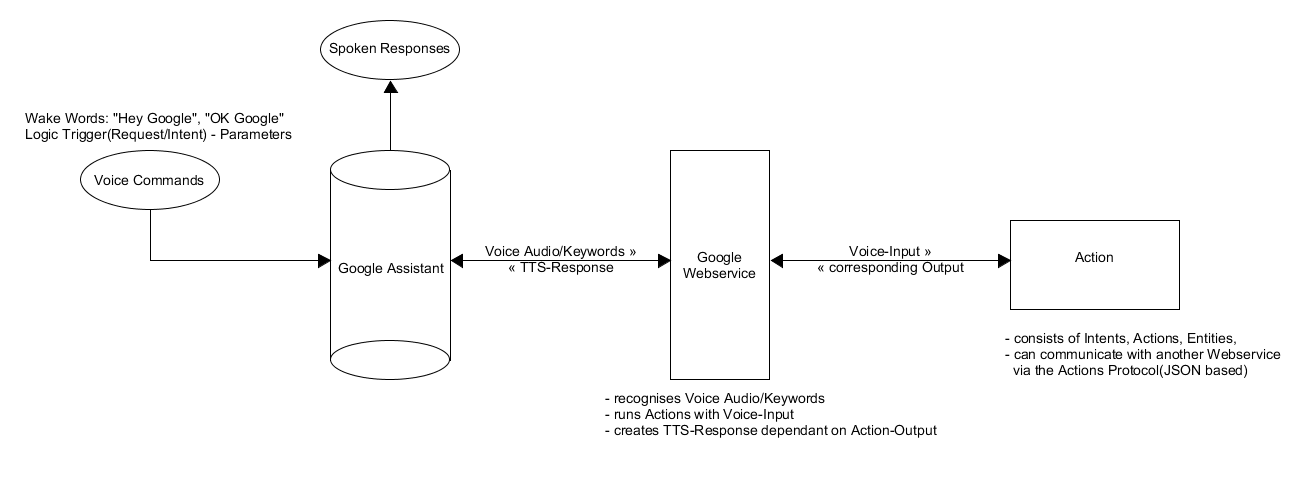
\includegraphics[width=0.9\textwidth]{content/img/GoogleVA_Architektur}
	\caption[Google Voice-Assistant Architektur]{Google Voice-Assistant Architektur}
\end{figure}
Der Google Assistant hat Zugriff auf Google Maps und kann daher Fragen zu Position örtlicher Geschäfte, sowie deren Öffnungszeiten beantworten. Generell steht dem Assistenten die Google Suche zur Verfügung um enzyklopedisches Wissen oder einfache Übersetzungen wiederzugeben.



\subsection{Hardware}

Es folgt ein kurzer Überblick über die verschiedenen Google Home Geräte, die momentan im Handel erhältlich sind.

\subsubsection{Google Home}
\begin{figure}[H]
	\begin{minipage}{0.45\textwidth}
	  \begin{itemize}
	  \item 149€
	  \item farbige Status-LEDs an der Oberfläche
	  \item kapazitiver Berührungssensor um Musik zu starten und stoppen oder die Lautstärke anzupassen
	  \item ein Mute-Button für das Mikrofon an der Rückseite
	  \end{itemize}
	\end{minipage}
	\hfill
	\begin{minipage}{0.45\textwidth}
	  \centering
	  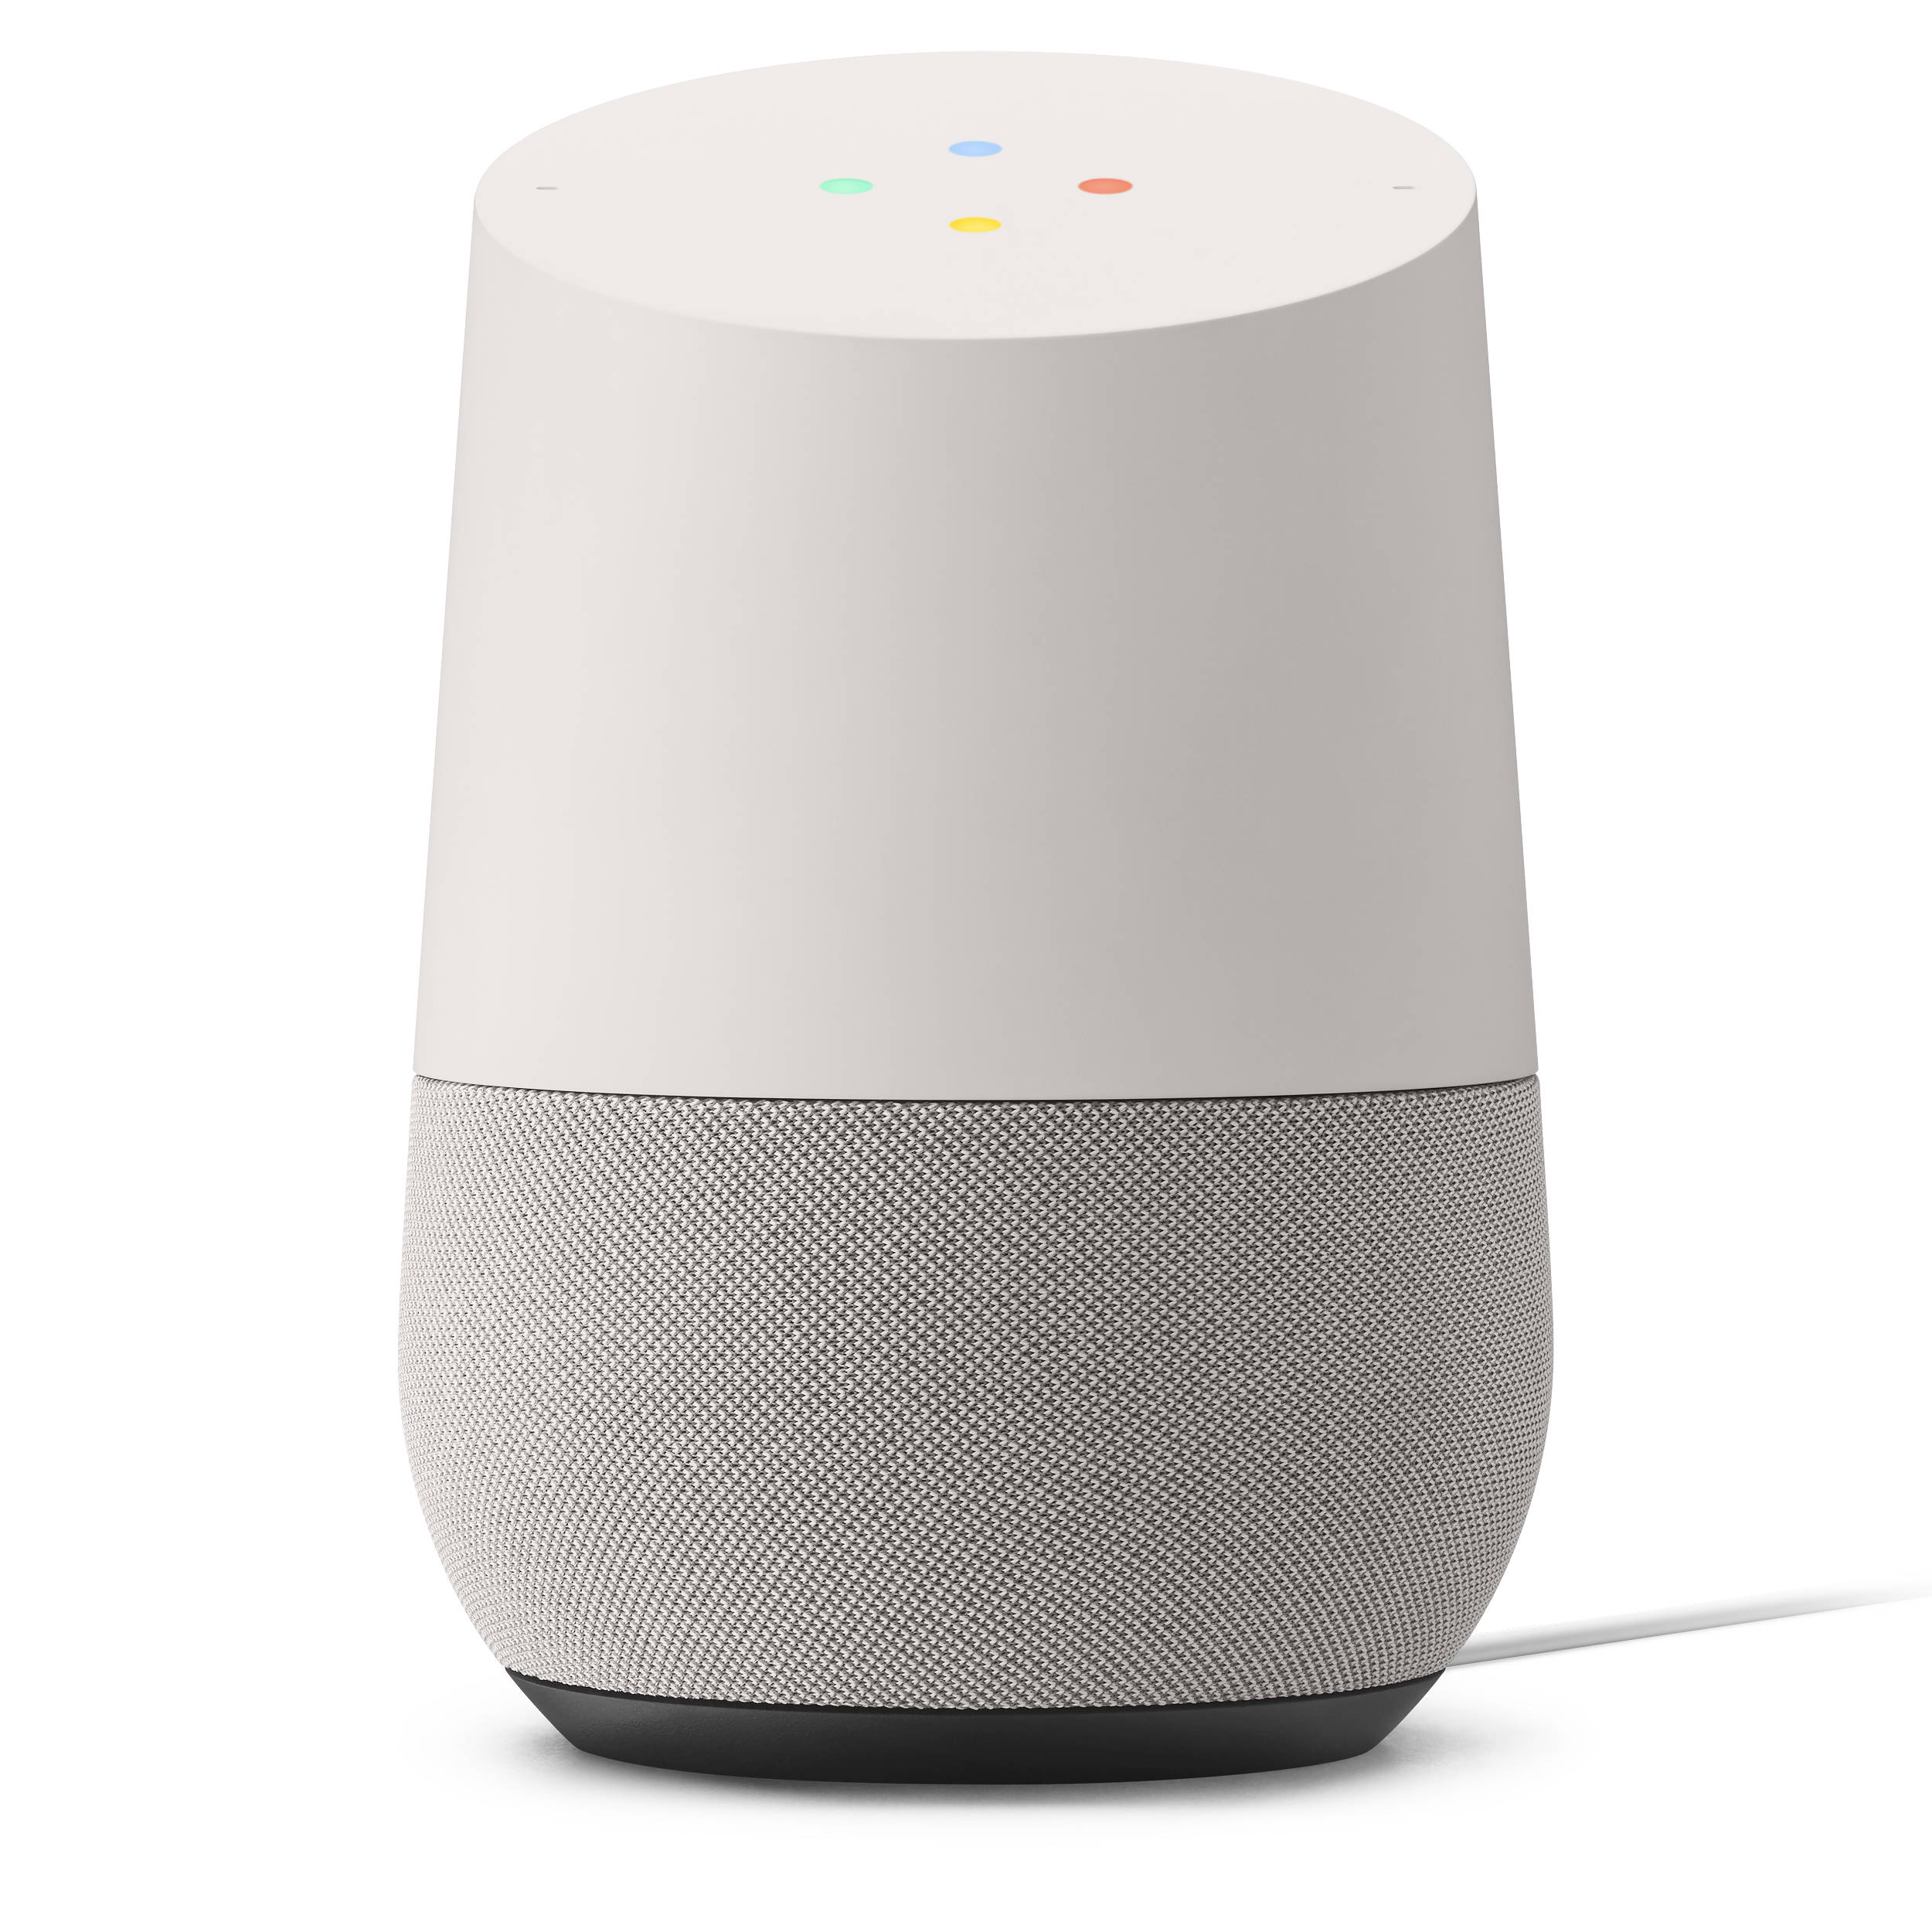
\includegraphics[width=\textwidth]{content/img/GoogleHome}
	  \caption[Google Home]{Google Home}
	\end{minipage}
\end{figure}

\subsubsection{Google Home Mini}
\begin{figure}[H]
	\begin{minipage}{0.45\textwidth}
	  \begin{itemize}
	  \item 59€
	  \item gleiche Funktionalität
	  \item Berührungssensor zum Anpassen der Lautstärke
	  \item weiße Statuslichter scheinen durch den Stoff auf der Oberseite
	  \item ein Mute-Schalter für das Mikrofon an der Rückseite
	  \end{itemize}
	\end{minipage}
	\hfill
	\begin{minipage}{0.45\textwidth}
	  \centering
      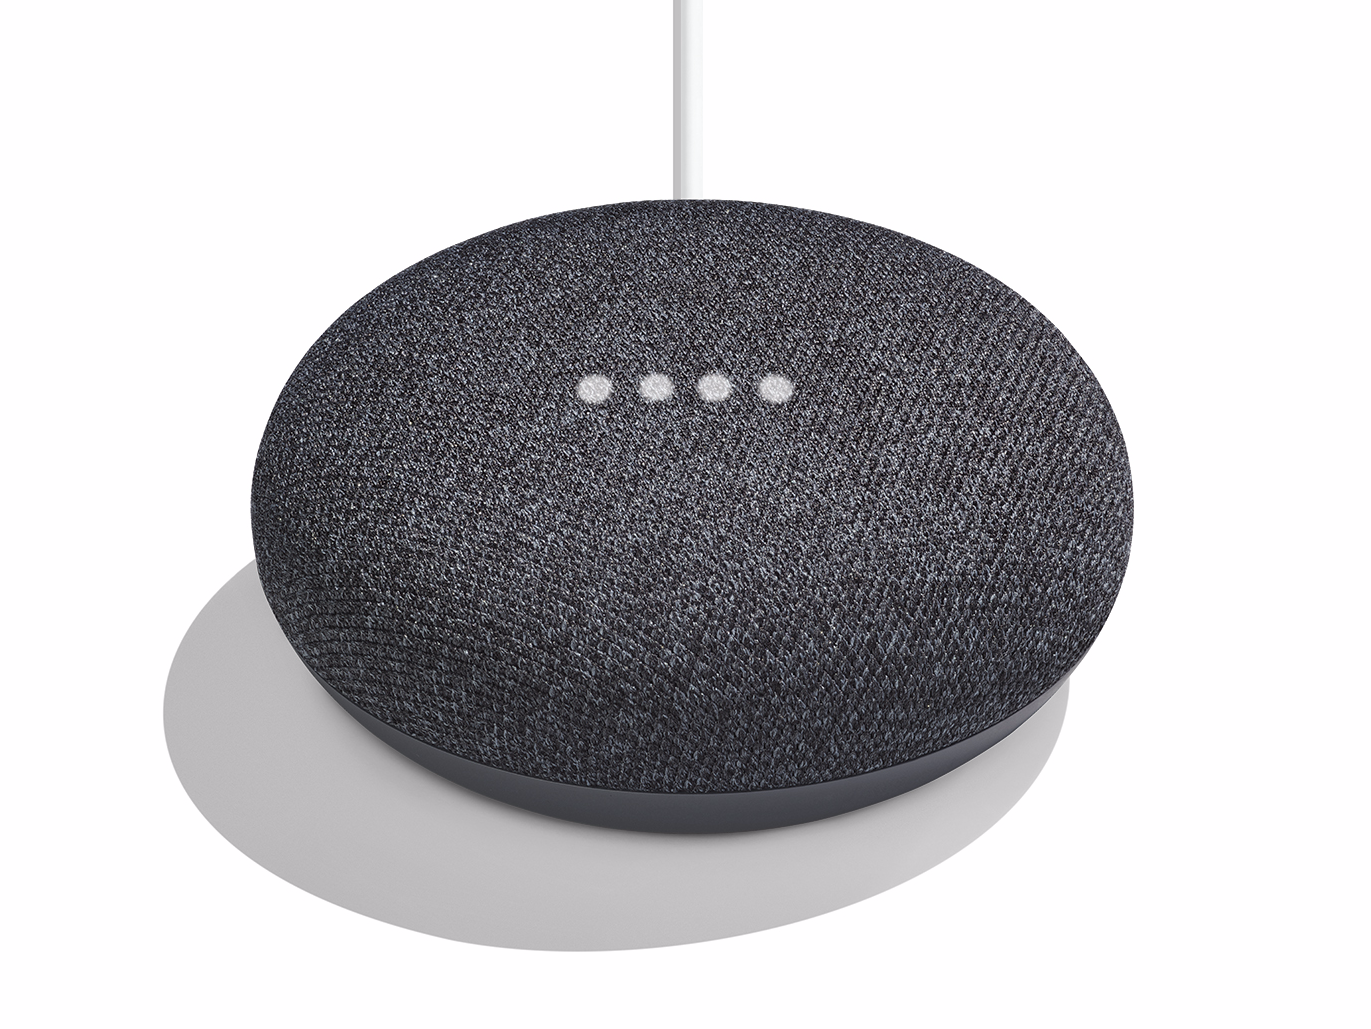
\includegraphics[width=\textwidth]{content/img/GoogleHomeMini}
      \caption[Google Home Mini]{Google Home Mini}
	\end{minipage}
\end{figure}

\subsubsection{Google Home Max}
\begin{figure}[H]
	\begin{minipage}{0.45\textwidth}
	  \begin{itemize}
	  \item 400\$
	  \item Stereo Lautsprecher(einschließlich zweier Hochtöner und Subwoofer)
	  \item magnetisch befestigbarer Ständer für vertikale Ausrichtung
	  \item beinhaltet \textit{Smart Sound}, ein Soundsystem das \textit{machine learning} nutzt um sich automatisch an die Umgebung anzupassen(Position und Geräuschquellen)
	  \end{itemize}
	\end{minipage}
	\hfill
	\begin{minipage}{0.45\textwidth}
	  \centering
      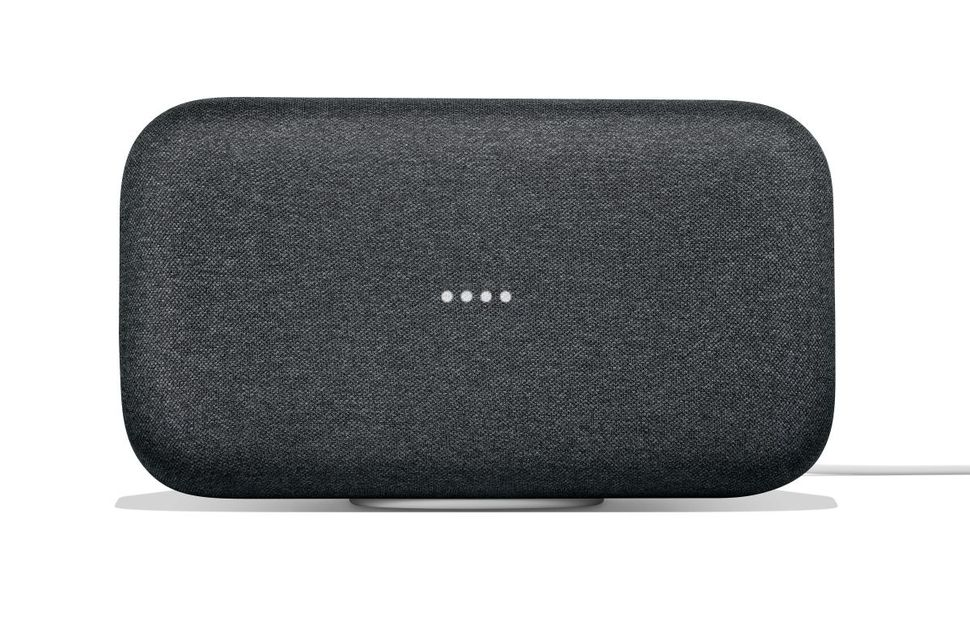
\includegraphics[width=\textwidth]{content/img/GoogleHomeMax}
      \caption[Google Home Max]{Google Home Max}
	\end{minipage}
\end{figure}

\subsection{Erweiterbarkeit}

Um eine App für den Google Assistant zu entwickeln bietet Google verschiedene Optionen.
Zum einen gibt es Templates, die einem einen Großteil der Programmierarbeit abnehmen und bereits vorgefertigte Konversationen enthalten. Allerdings gibt es bisher nicht viele Templates aus denen man wählen kann.\\
Für einfache Apps mit wenig Inputmöglichkeiten bietet sich die \textit{Actions SDK} an. Sie bietet keine NLU (natural language understanding), es kann allerdings eine eigene NLU eigesetzt werden.
Weiterhin müssen \textit{action packages} mit einem Text Editor geschrieben und per Kommando-Zeilen Tool an das jeweilige Google Developer Projekt gesendet werden.\\
\textit{Dialogflow} ist eine Web IDE, die die Funktionalität der \textit{Actions SDK} einschließt.
\textit{Dialogflow} beinhaltet eine \textit{NLU engine} die natürliche, menschliche Sprache parsen kann.

\subsection{Actions}

Im Folgenden wird auf den Aufbau der Actions in Dialogflow eingegangen.\\
Intents sind ein Hauptbestandteil der Actions. Sie werden mithilfe von \textit{machine learning} von Dialogflow aus \textit{Utterances} (Äußerungen des Nutzers) bestimmt. Die Intents können mehrere Parameter enthalten. Diese können von der \textit{NLU engine} als Entities erkannt werden.\\
Entities sind Tabellen in denen Einträge von Objekten eines Typs vordefiniert werden können.
Zur Unterstützung der Spracherkennung können Synonyme für die Objekte eigetragen werden.
Sie dienen zur Erkennung von relevanten Daten in den Intents.\\
Als Antwort auf ein Intent kann eine Text Response zurückgegeben werden. Unter dem Menüpunkt Fullfilment kann allerdings auch auf einen Webservice verlinkt werden, an den geparste Intents über das \textit{Actions Protocol} (JSON basiert) versendet werden. Der Webservice kann daraufhin den Inhalt auswerten und eine Antwort zurücksenden, die dann von der Action zurückgegeben werden kann.